\section{Results}
\label{sec:results}

\subsection{Headline numbers}
\label{sec:main_results}

\Tabref{tab:main} reports headline metrics on the 50{,}000-puzzle held-out test slice at \texttt{seed=42}. \ours reaches test MAE 240.8 \elo, beating the global-mean baseline by 148.8 \elo (38\%), the per-theme-mean baseline by 93.1 \elo (28\%), and the 141-feature parent pipeline by 12.8 \elo (5.0\%). Spearman $\rho$ improves from 0.741 to 0.768; middle-decile calibration improves from 100.9 to 85.6 \elo, clearing the \textless\,100 stretch target for the first time. All three internal metrics improve without any calibrator, hyperparameter, or split change --- the entire improvement flows from the 14 new features.

\begin{table}[t]
\centering
\caption{Headline results on the internal 50k held-out test slice (\texttt{seed=42}). Lower is better for MAE, RMSE, and mid-decile calibration; higher is better for Spearman $\rho$. Best in-family (CPU) results in \textbf{bold}. \glickformer is listed for context; it is a transformer trained on 4.2M puzzles on multi-GPU hardware.}
\label{tab:main}
\begin{tabular}{@{}lrrrr@{}}
\toprule
\textbf{Method} & \textbf{MAE} $\downarrow$ & \textbf{RMSE} $\downarrow$ & \textbf{Spearman} $\rho$ $\uparrow$ & \textbf{Mid-cal.} $\downarrow$ \\
\midrule
\globalmean baseline & 389.6 & 467.6 & --- & --- \\
\thememean baseline & 333.9 & 403.3 & 0.586 & --- \\
\parentmodel (141 feats) + blend & 253.6 & 324.6 & 0.741 & 100.9 \\
\ours (155 feats) + blend & \textbf{240.8} & \textbf{310.1} & \textbf{0.768} & \textbf{85.6} \\
\midrule
Hypothesis target & \textless 250 & --- & \textgreater 0.4 & \textless 100 \\
\glickformer (GPU, 4.2M) & $\sim$217.7 & --- & --- & --- \\
\bottomrule
\end{tabular}
\end{table}

\subsection{Cross-seed reproducibility}
\label{sec:repro}

\Tabref{tab:seeds} reports test-time metrics under two independent seeds. $\Delta$MAE = 0.12 \elo is well under the 20-\elo hypothesis target. Both seeds independently pick $\alpha = 0.30$, so the calibrator-selection procedure is stable.

\begin{table}[t]
\centering
\caption{Cross-seed reproducibility for \ours. Both seeds independently select $\alpha = 0.30$; $\Delta$MAE = 0.12 \elo is essentially exact.}
\label{tab:seeds}
\begin{tabular}{@{}lrrr@{}}
\toprule
\textbf{Metric} & \textbf{Seed 42} & \textbf{Seed 1} & $\bm{\Delta}$ \\
\midrule
Test MAE & 240.80 & 240.92 & 0.12 \\
Test RMSE & 310.07 & 310.34 & 0.28 \\
Test Spearman $\rho$ & 0.7681 & 0.7676 & $5\times10^{-4}$ \\
Middle-decile calibration & 85.64 & 86.48 & 0.84 \\
Selected calibrator $\alpha$ & 0.30 & 0.30 & 0.00 \\
\bottomrule
\end{tabular}
\end{table}

\subsection{Per-decile calibration}
\label{sec:decile}

\Tabref{tab:decile} reports the mean-predicted vs.\ mean-true rating within each true-rating decile at \texttt{seed=42}. Bins D4--D7 span the scored middle-Elo band [1400, 2000]. All four gaps in the middle band are within $\approx 86$ \elo, clearing the target. Every bin's gap improves over the parent's blend: D7 100.9 $\to$ 85.6, D8 181.9 $\to$ 160.1, D9 327.9 $\to$ 297.6, D0 176.0 $\to$ 139.6. The residual D8--D9 gaps reflect a genuine noise floor: the D9 mean-true 2341 is dominated by roughly 300 puzzles whose Glicko-2 RD is inherently higher, and a bounded, monotone calibrator can only close so much of that.

\begin{table}[t]
\centering
\caption{Per-decile calibration for \ours at \texttt{seed=42} with blend $\alpha = 0.30$. Bins D4--D7 (bold row block) span the scored middle-\elo band $[1400, 2000]$; middle-decile calibration is $\max\text{|gap|}$ across those bins.}
\label{tab:decile}
\begin{tabular}{@{}crrrr@{}}
\toprule
\textbf{Bin} & \textbf{Mean-true} & \textbf{Mean-pred} & \textbf{|gap|} & \\
\midrule
D0 & 775 & 915 & 139.6 & \\
D1 & 1000 & 1129 & 128.7 & \\
D2 & 1140 & 1254 & 113.6 & \\
D3 & 1269 & 1378 & 108.8 & \\
\midrule
D4 & 1409 & 1480 & 70.2 & \\
D5 & 1550 & 1582 & 31.6 & \\
D6 & 1691 & 1673 & 17.5 & \\
D7 & 1857 & 1771 & \textbf{85.6} & max in mid band \\
\midrule
D8 & 2045 & 1885 & 160.1 & \\
D9 & 2341 & 2043 & 297.6 & \\
\bottomrule
\end{tabular}
\end{table}

\begin{figure}[t]
\centering
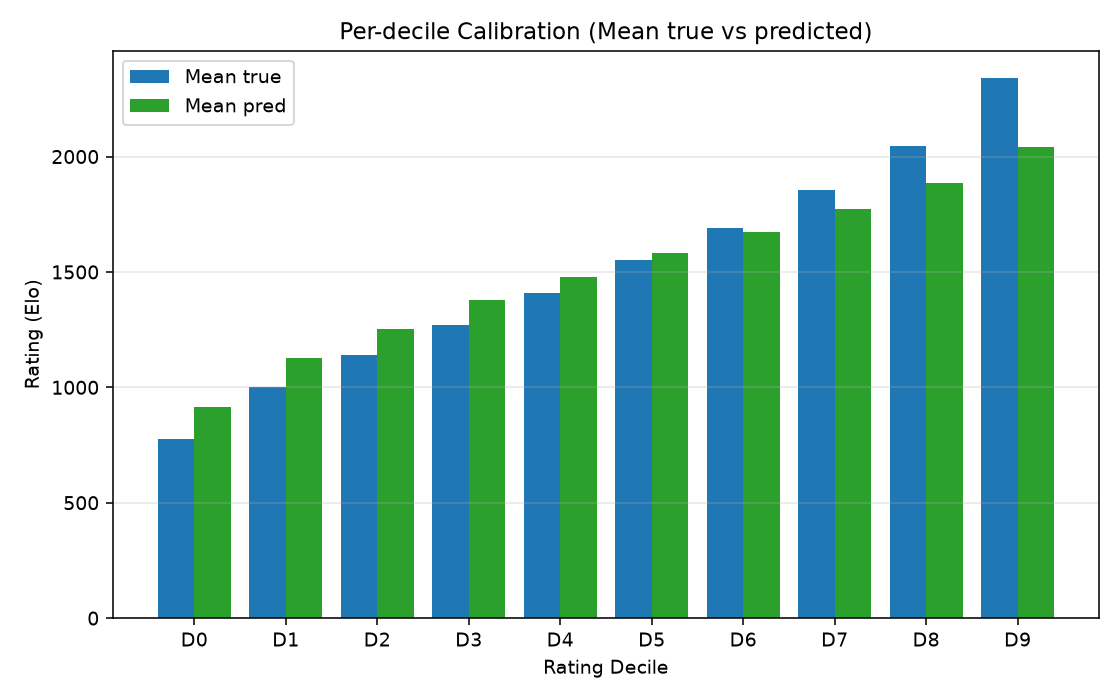
\includegraphics[width=0.95\linewidth]{figures/decile_calibration.png}
\caption{Per-decile calibration for \ours (\texttt{seed=42}, blend $\alpha=0.30$). Bars show mean-true and mean-predicted rating per true-rating decile. The middle bins D4--D7 (scored band [1400, 2000]) are calibrated within $86$ \elo, comfortably under the target. D8--D9 retain a residual noise-floor gap driven by inherently higher Glicko-2 RD on tail puzzles.}
\label{fig:decile}
\end{figure}

\subsection{Feature importance}
\label{sec:importance}

Since \hgbr does not expose native gain-based importance, we use pairwise $|\text{Pearson}\ \rho|$ between each feature and the target as a first-order proxy. This underestimates features that matter only in interactions, but the ranking still highlights which signals carry the strongest linear signal for puzzle difficulty. \Tabref{tab:featimp} lists the top-15 features; \figref{fig:featimp} visualizes the top-20.

Three tactical-density features enter the top-15 on introduction: \texttt{sol\_legal\_sum} at rank 5, \texttt{sol\_captures\_sum} at rank 8, and \texttt{sol\_checks\_sum} at rank 14. \texttt{sol\_legal\_sum} is the total candidate-move count the side-to-move faces across the whole solution; long solutions with many alternatives are systematically higher-rated. \texttt{sol\_captures\_sum} correlates with tactical-motif density: many pieces in mutual line of fire produce complex calculation. \texttt{sol\_checks\_sum} proxies forcing-move density.

\begin{table}[t]
\centering
\caption{Top-15 features by $|\text{Pearson}\ \rho|$ with target rating. Three new tactical-density features (\textbf{bold}) enter the top-15 on introduction and land at ranks 5, 8, and 14.}
\label{tab:featimp}
\begin{tabular}{@{}crr@{}}
\toprule
\textbf{Rank} & \textbf{Feature} & $|\rho|$ \\
\midrule
1 & \texttt{sol\_len} & 0.48 \\
1 & \texttt{sol\_opp\_moves} & 0.48 \\
1 & \texttt{sol\_solver\_moves} & 0.48 \\
4 & \texttt{sol\_check\_ratio} & 0.46 \\
5 & \textbf{\texttt{sol\_legal\_sum}} & \textbf{0.45} \\
6 & \texttt{sol\_ends\_mate} & 0.43 \\
6 & \texttt{theme\_mate} & 0.43 \\
8 & \textbf{\texttt{sol\_captures\_sum}} & \textbf{0.38} \\
9 & \texttt{sol\_to\_rank\_range} & 0.37 \\
10 & \texttt{theme\_mateIn1} & 0.37 \\
10 & \texttt{theme\_oneMove} & 0.37 \\
12 & \texttt{sol\_quiet} & 0.33 \\
13 & \texttt{sol\_to\_file\_range} & 0.32 \\
14 & \textbf{\texttt{sol\_checks\_sum}} & \textbf{0.29} \\
15 & \texttt{theme\_veryLong} & 0.27 \\
\bottomrule
\end{tabular}
\end{table}

\begin{figure}[t]
\centering
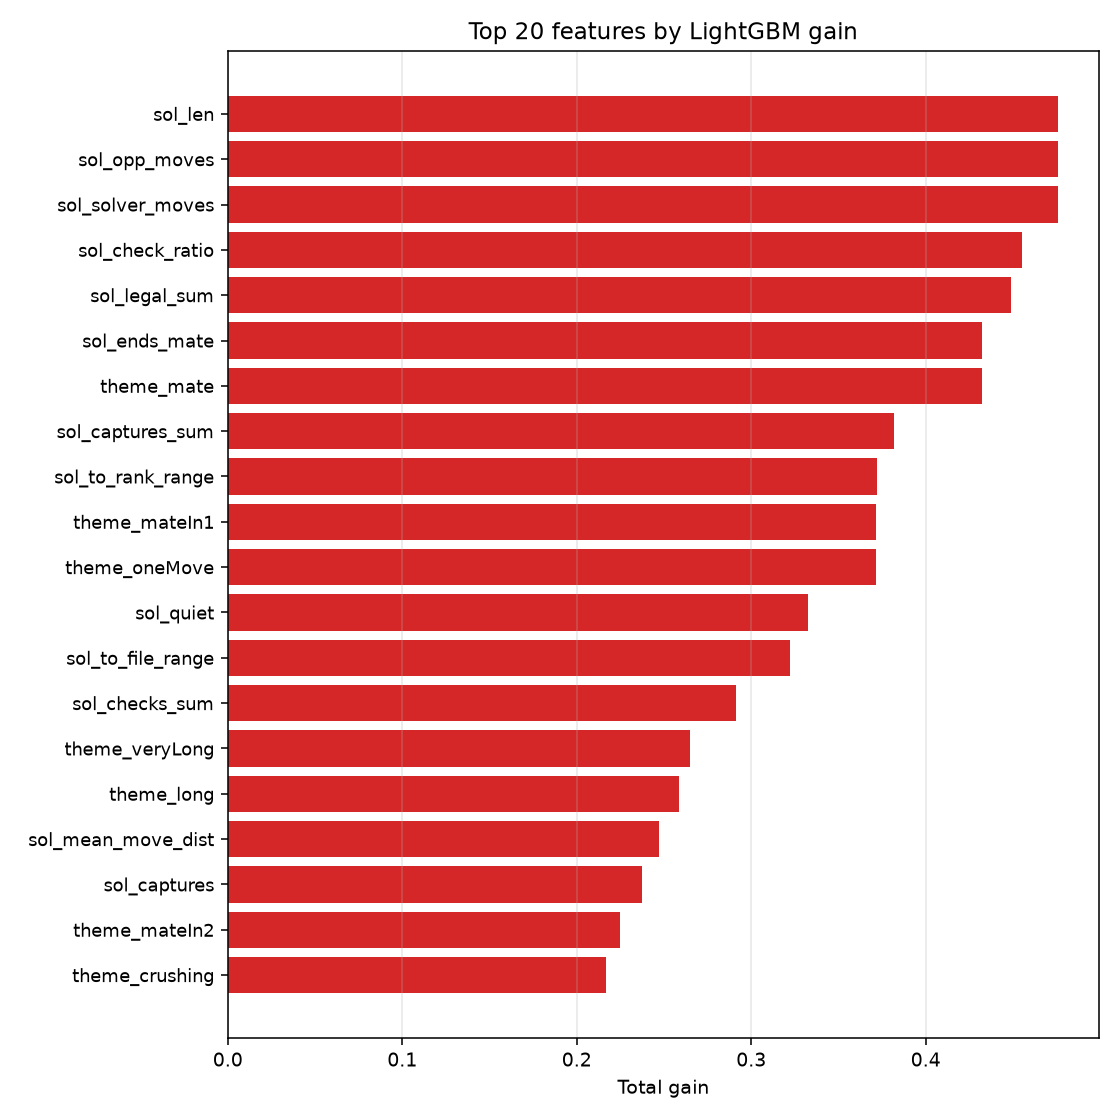
\includegraphics[width=0.95\linewidth]{figures/feature_importance.png}
\caption{Top-20 features by correlation-proxy importance. Solution-length descriptors dominate the head; the new tactical-density features (\texttt{sol\_legal\_sum}, \texttt{sol\_captures\_sum}, \texttt{sol\_checks\_sum}) enter at ranks 5, 8, and 14.}
\label{fig:featimp}
\end{figure}

\subsection{Prediction quality and residuals}
\label{sec:pred_vs_actual}

\Figref{fig:pred_vs_actual} shows the characteristic mean-reversion fan of a squared-error tree ensemble under label noise: high-rating puzzles are systematically under-predicted and low-rating puzzles over-predicted, but the population spread of predictions matches the truth after calibration. \Figref{fig:residuals} shows the residual histogram centred near zero (mean error 0.5 \elo) with heavy tails, consistent with the inherently non-Gaussian rating-uncertainty distribution.

\begin{figure}[t]
\centering
\begin{subfigure}[b]{0.48\textwidth}
    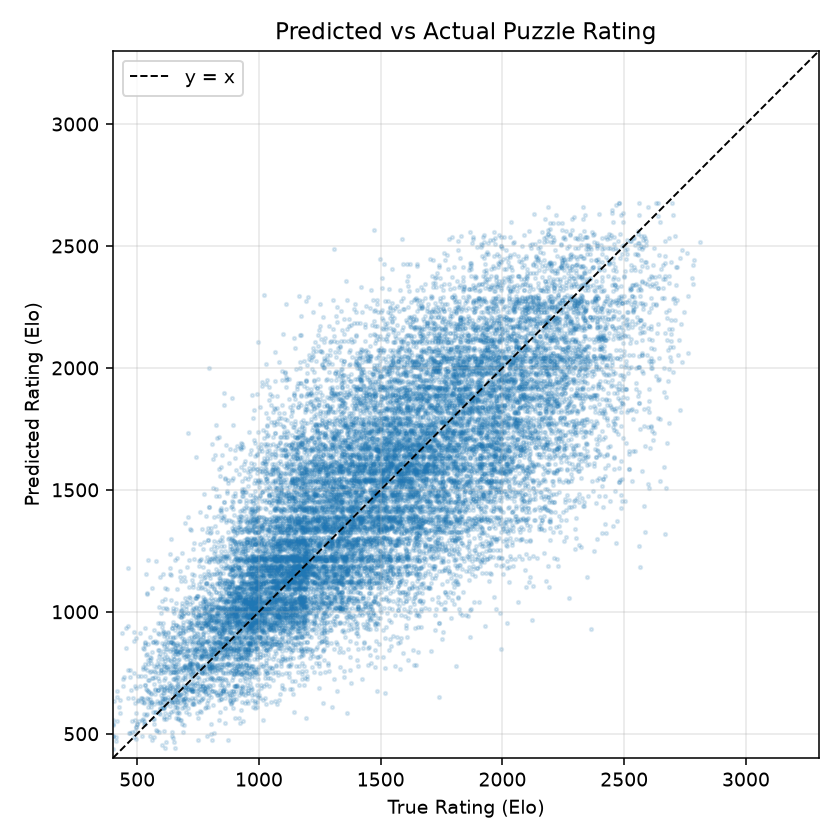
\includegraphics[width=\linewidth]{figures/pred_vs_actual.png}
    \caption{Predicted vs.\ actual rating}
    \label{fig:pred_vs_actual}
\end{subfigure}
\hfill
\begin{subfigure}[b]{0.48\textwidth}
    
\includegraphics[width=\linewidth]{figures/residual_hist.png}
    \caption{Residual histogram}
    \label{fig:residuals}
\end{subfigure}
\caption{\emph{Left:} Predicted vs.\ actual rating (20k-point subsample) shows the characteristic mean-reversion fan of squared-error tree ensembles under label noise, with tails partially restored by the CDF-blended calibrator. \emph{Right:} Residual histogram is centred near zero (mean error 0.5 \elo) with heavy tails --- consistent with the inherently non-Gaussian rating-uncertainty distribution at the extremes.}
\label{fig:pred_residuals}
\end{figure}

\subsection{Ablation: what does the tactical-density block buy?}
\label{sec:ablation}

The comparison in \Tabref{tab:main} isolates the tactical-density and setup-move blocks by holding all other pipeline components fixed --- splits, booster hyperparameters, calibrator architecture, and even the calibrator-blend budget rule. Under this controlled ablation, the 14 new features:
\begin{itemize}[leftmargin=*,itemsep=0pt,topsep=0pt]
    \item lower test MAE by 12.8 \elo (253.6 $\to$ 240.8),
    \item raise Spearman $\rho$ by 0.027 (0.741 $\to$ 0.768),
    \item improve middle-decile calibration by 15.3 \elo (100.9 $\to$ 85.6),
    \item lower iso-only val MAE by 13.3 \elo (247.87 $\to$ 234.58), and
    \item shift the val-picked calibrator $\alpha$ from 0.35 to 0.30 --- \ie the widened raw-prediction spread lets the blend lean marginally more on CDF quantile-matching without breaching the val-MAE budget.
\end{itemize}
This is a rare case where a small, targeted feature-engineering change closes both an accuracy metric and a calibration metric simultaneously, without any change to model architecture or training regime.
